\section{シミュレーションワールドの構成}
\label{sec:sim_world}

本節では，本研究で用いたシミュレーションワールドの構成について述べる．シミュレーションワールドは，ロボットが歩行中に足を接地する位置のみに足場を配置した (\cref{fig:world})，いわゆる飛び石状の地形として構成した．各足場は歩行計画に基づく接地位置に対応して配置されており，ロボットが意図した位置に確実に足を下ろす状況を再現することを目的としている．これにより，床特性以外の要因が歩行挙動に影響を与えないよう配慮した．

配置された足場のうち，一か所のみを軟弱地面として設定し，ロボットが踏み込んだ際に鉛直方向へ沈み込みが生じる床モデルを導入した．その他の足場は剛体床とし，沈み込みは生じない．このように単一の沈み込み床を含むワールド構成とすることで，床沈み込みが歩行挙動に与える影響を局所的かつ明確に観測できるようにしている．

\begin{figure}[htbp]
  \centering
  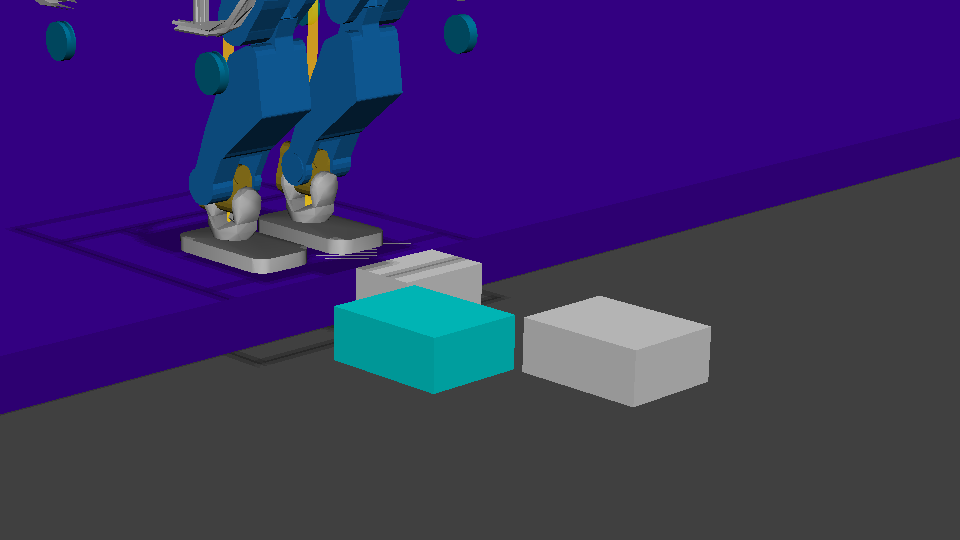
\includegraphics[width=0.5\linewidth]{images/world.png}
  \caption{飛び石状のシミュレーションワールド}
  \label{fig:world}
\end{figure}

\subsection{床モデルおよび条件分けの方針}
\label{subsec:floor_model_policy}

軟弱地面は，鉛直方向にのみ変位可能な床要素としてモデル化し，その力学特性を一次元のバネ・マス・ダンパー系として表現した．本研究では条件を簡単にするため，床は常に平行であるものとし，回転や傾斜は考慮しない．床に加わる反力は，床の沈み込み量および沈み込み速度に応じて決定され，バネ定数およびダンパー定数によって床の剛性および減衰特性が規定される．

床物理特性の違いが歩行挙動に与える影響を体系的に評価するため，本研究では床条件を合計4種類設定した．このうち3種類は実環境に存在するスポンジ材料を対象とした物理特性測定に基づく条件であり，残り1種類はシミュレーション上において従来手法による歩行が限界的に不安定化する条件として設定した．これにより，実環境に近い床条件から制御限界に近い条件までを含めた評価を可能としている．実環境に存在する材料として，本研究では高反発・低反発ウレタン及び緩衝材用のスポンジを使用した．

\subsection{実環境における床物理特性の測定概要}
\label{subsec:floor_measurement}

実環境の床物理特性の測定には，産業用マニピュレータ UR5e の先端に実際に本研究で使用しているロボットの足首についている6軸力覚センサを取り付けた計測系を用いた (\cref{fig:ur5e_sensor})．測定対象となるスポンジ材料に対して，アーム先端を鉛直方向に押し付け，その際に得られる反力および変位履歴を計測した．

UR5e は，先端に加わる力が約150\,Nを超えた場合に緊急停止する安全機構を備えている．そのため，本測定では反力が150\,Nを超えない範囲に押し込み量を制限し，材料の上面付近のみを対象として測定を行った．この制約の下で，押し込み量を一定とし，押し込みに要する時間を0.5秒から3.0秒まで0.5秒刻みで変化させた計6パターンの測定を実施した．

\begin{figure}[htbp]
  \centering
  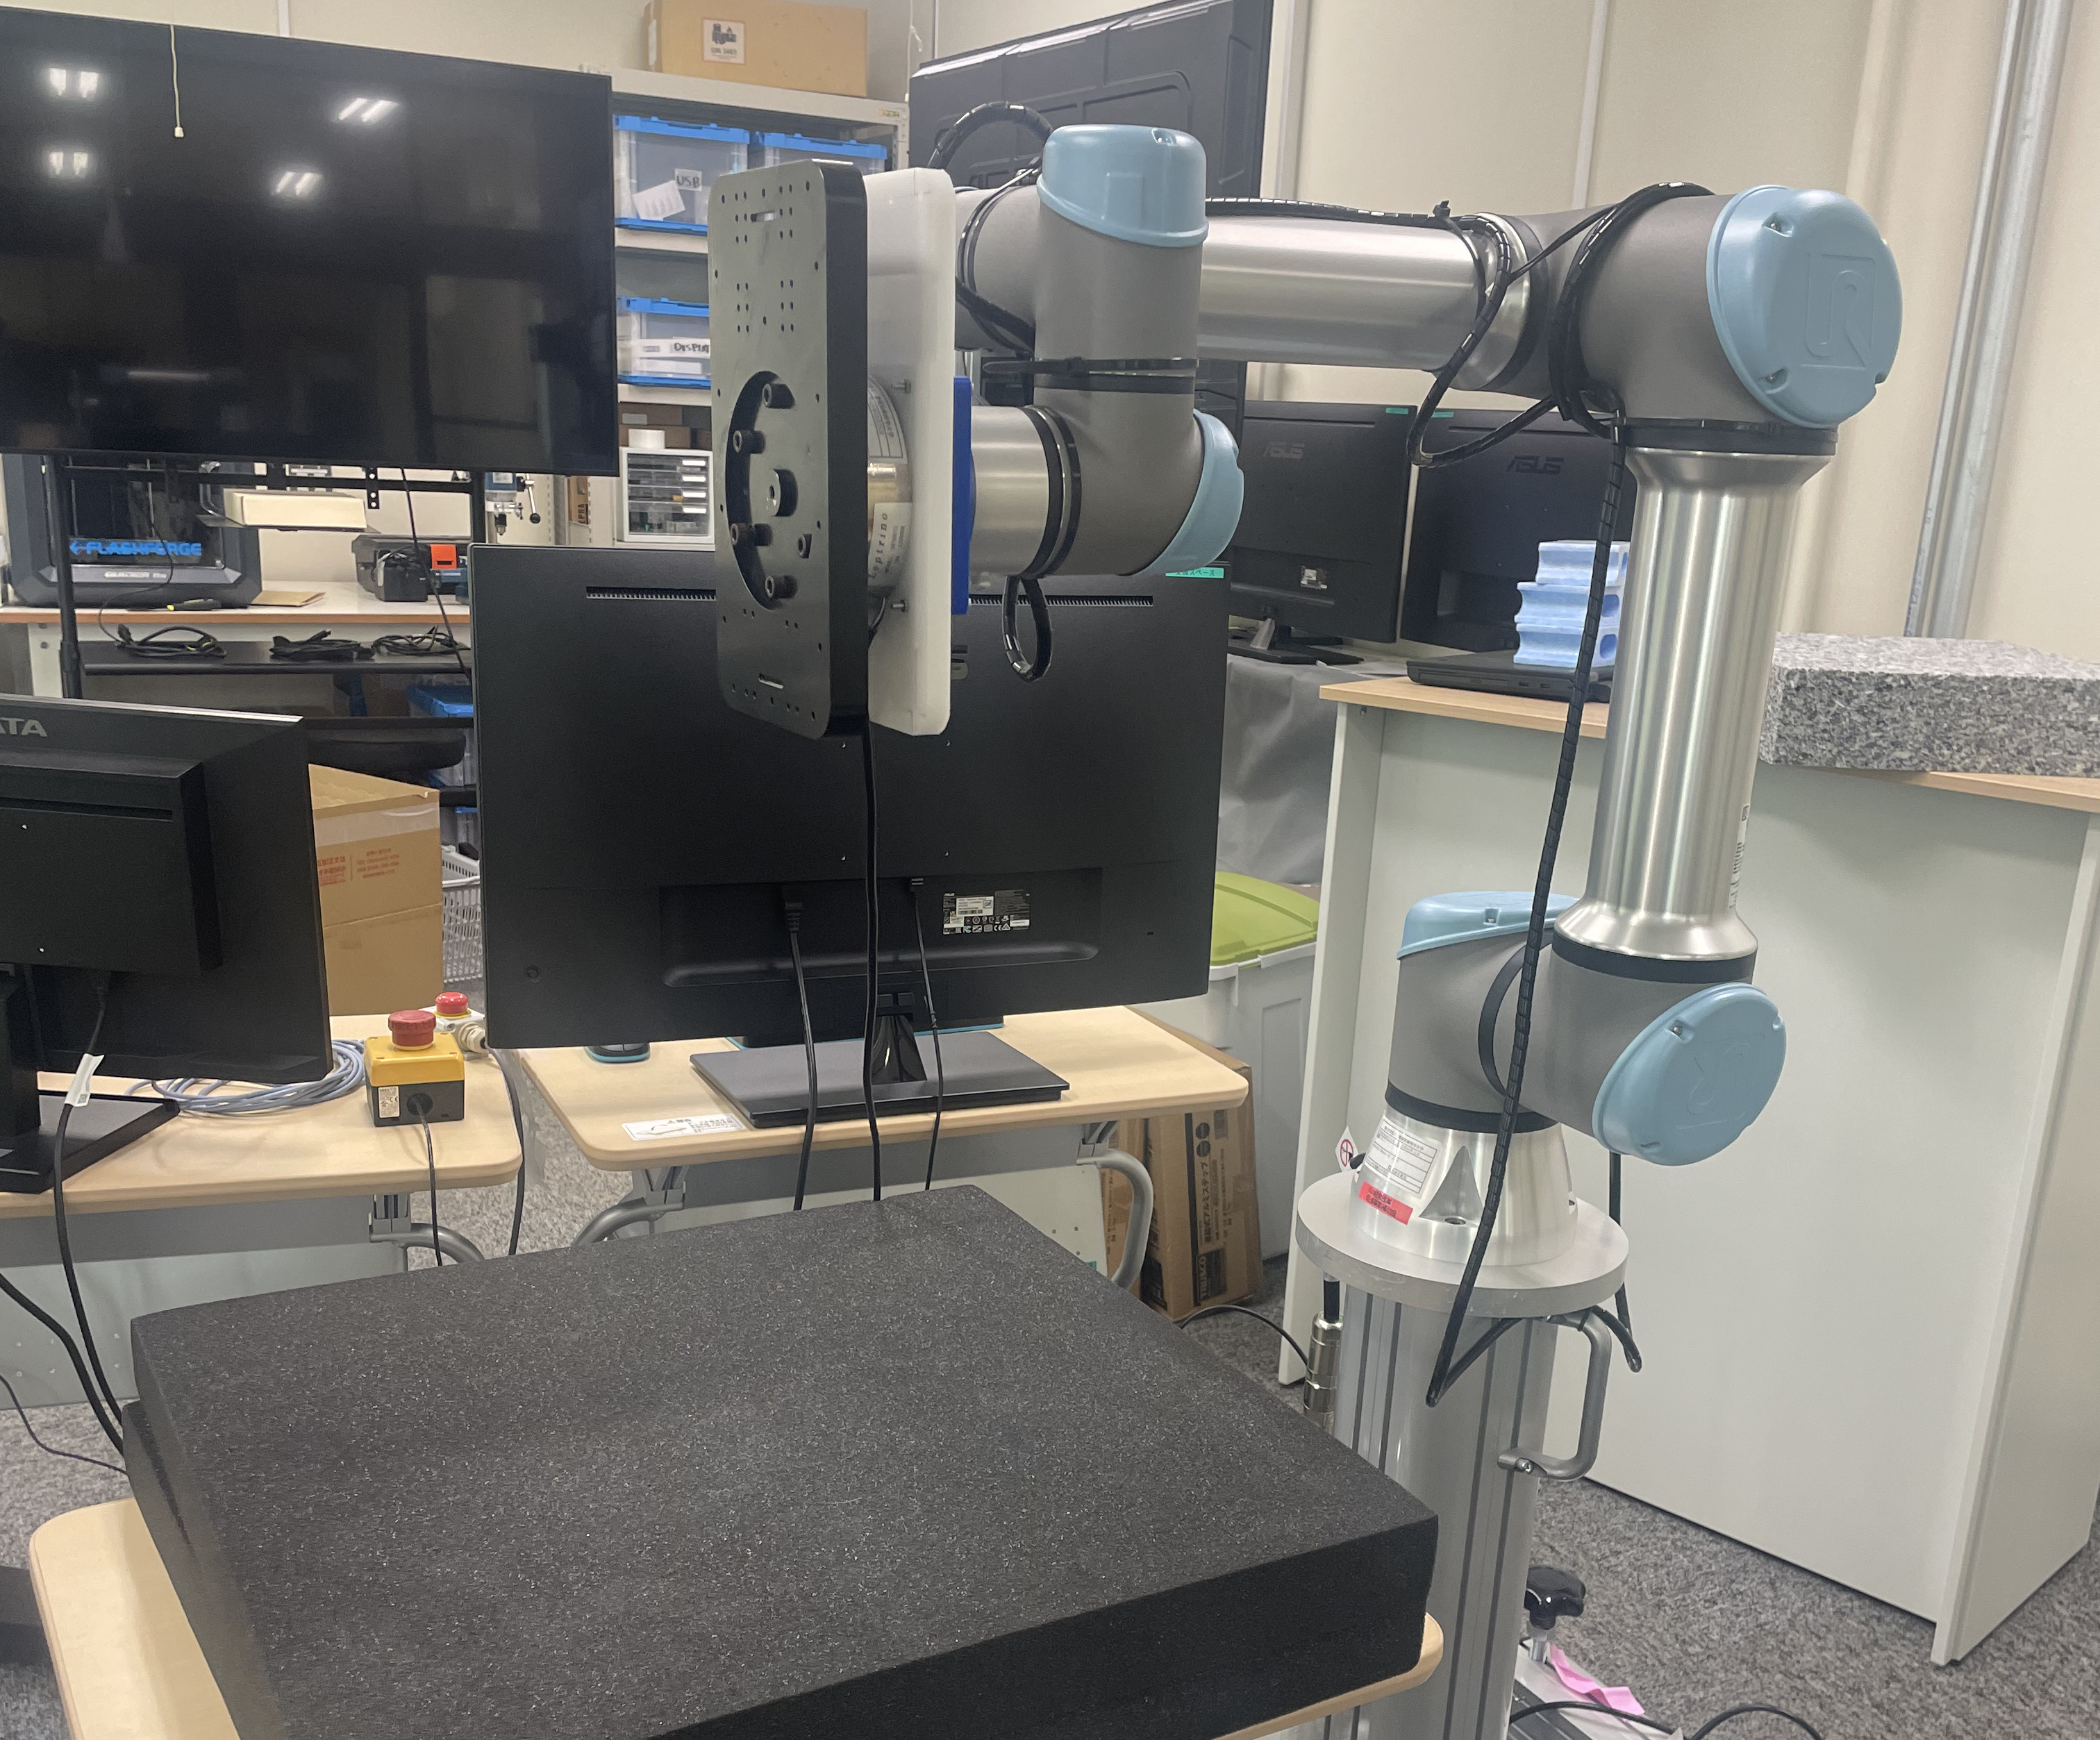
\includegraphics[width=0.5\linewidth]{images/ur5e_sensor.png}
  \caption{UR5eマニピュレータと力覚センサ}
  \label{fig:ur5e_sensor}
\end{figure}

\subsection{床物理特性の近似モデル}
\label{subsec:floor_identification}

床の鉛直方向の力学特性は，バネマスダンパー系に基づく Kelvin--Voigt 型モデルとして近似した．床は鉛直方向にのみ変位する一次元要素として扱い，押し込み変位 $x$ およびその速度 $\dot{x}$ に対して反力 $F$ が線形に発生するものと仮定した．床反力は次式で表される．
\begin{equation}
F(t)=k\,x(t)+c\,\dot{x}(t),
\label{eq:kv_model}
\end{equation}
ここで $k$ はバネ定数 [N/m]，$c$ はダンパー定数 [N$\cdot$s/m] である．

押し込み量を一定とし，押し込みに要する時間を変化させることで異なる速度条件を与えた．押し込み量を $x_{\mathrm{total}}$，押し込み時間を $T$ とすると，押し込み速度は
\begin{equation}
v=\frac{x_{\mathrm{total}}}{T}
\end{equation}
と表される．押し込み区間では変位が時間に対して線形に増加するものと仮定し，測定された反力データに対して最小二乗法を適用することで，各床条件に対応するバネ定数およびダンパー定数を推定した．

\subsection{シミュレーションに用いた床物理パラメータ}
\label{subsec:floor_params}

測定結果を用いて近似した結果を \cref{tab:floor_params} に示す．Case~1 および Case~2 は高反発および低反発ウレタンに対応する条件，Case~3 は緩衝材用スポンジに対応する条件である．Case~4 は，シミュレーション上で従来手法による歩行が限界的に不安定化するよう設定した床条件である．これらの条件を用いることで，床物理特性の違いが歩行挙動に与える影響を比較評価した．

\begin{table}[t]
  \centering
  \caption{シミュレーションに用いた床物理パラメータ}
  \label{tab:floor_params}
  \begin{tabular}{c c c c}
    \hline
    条件 & 由来 & バネ定数 $K$ [N/m] & ダンパー定数 $D$ [Ns/m] \\
    \hline
    Case~1 & 高反発ウレタン & $29{,}254$ & $619$ \\
    Case~2 & 低反発ウレタン & $30{,}395$ & $2{,}289$ \\
    Case~3 & 緩衝材用スポンジ & $4{,}125$ & $1{,}021$ \\
    Case~4 & シミュレーション設定床 & $7{,}000$ & $2{,}000$ \\
    \hline
  \end{tabular}
\end{table}

\begin{figure}[htbp]
  \centering
  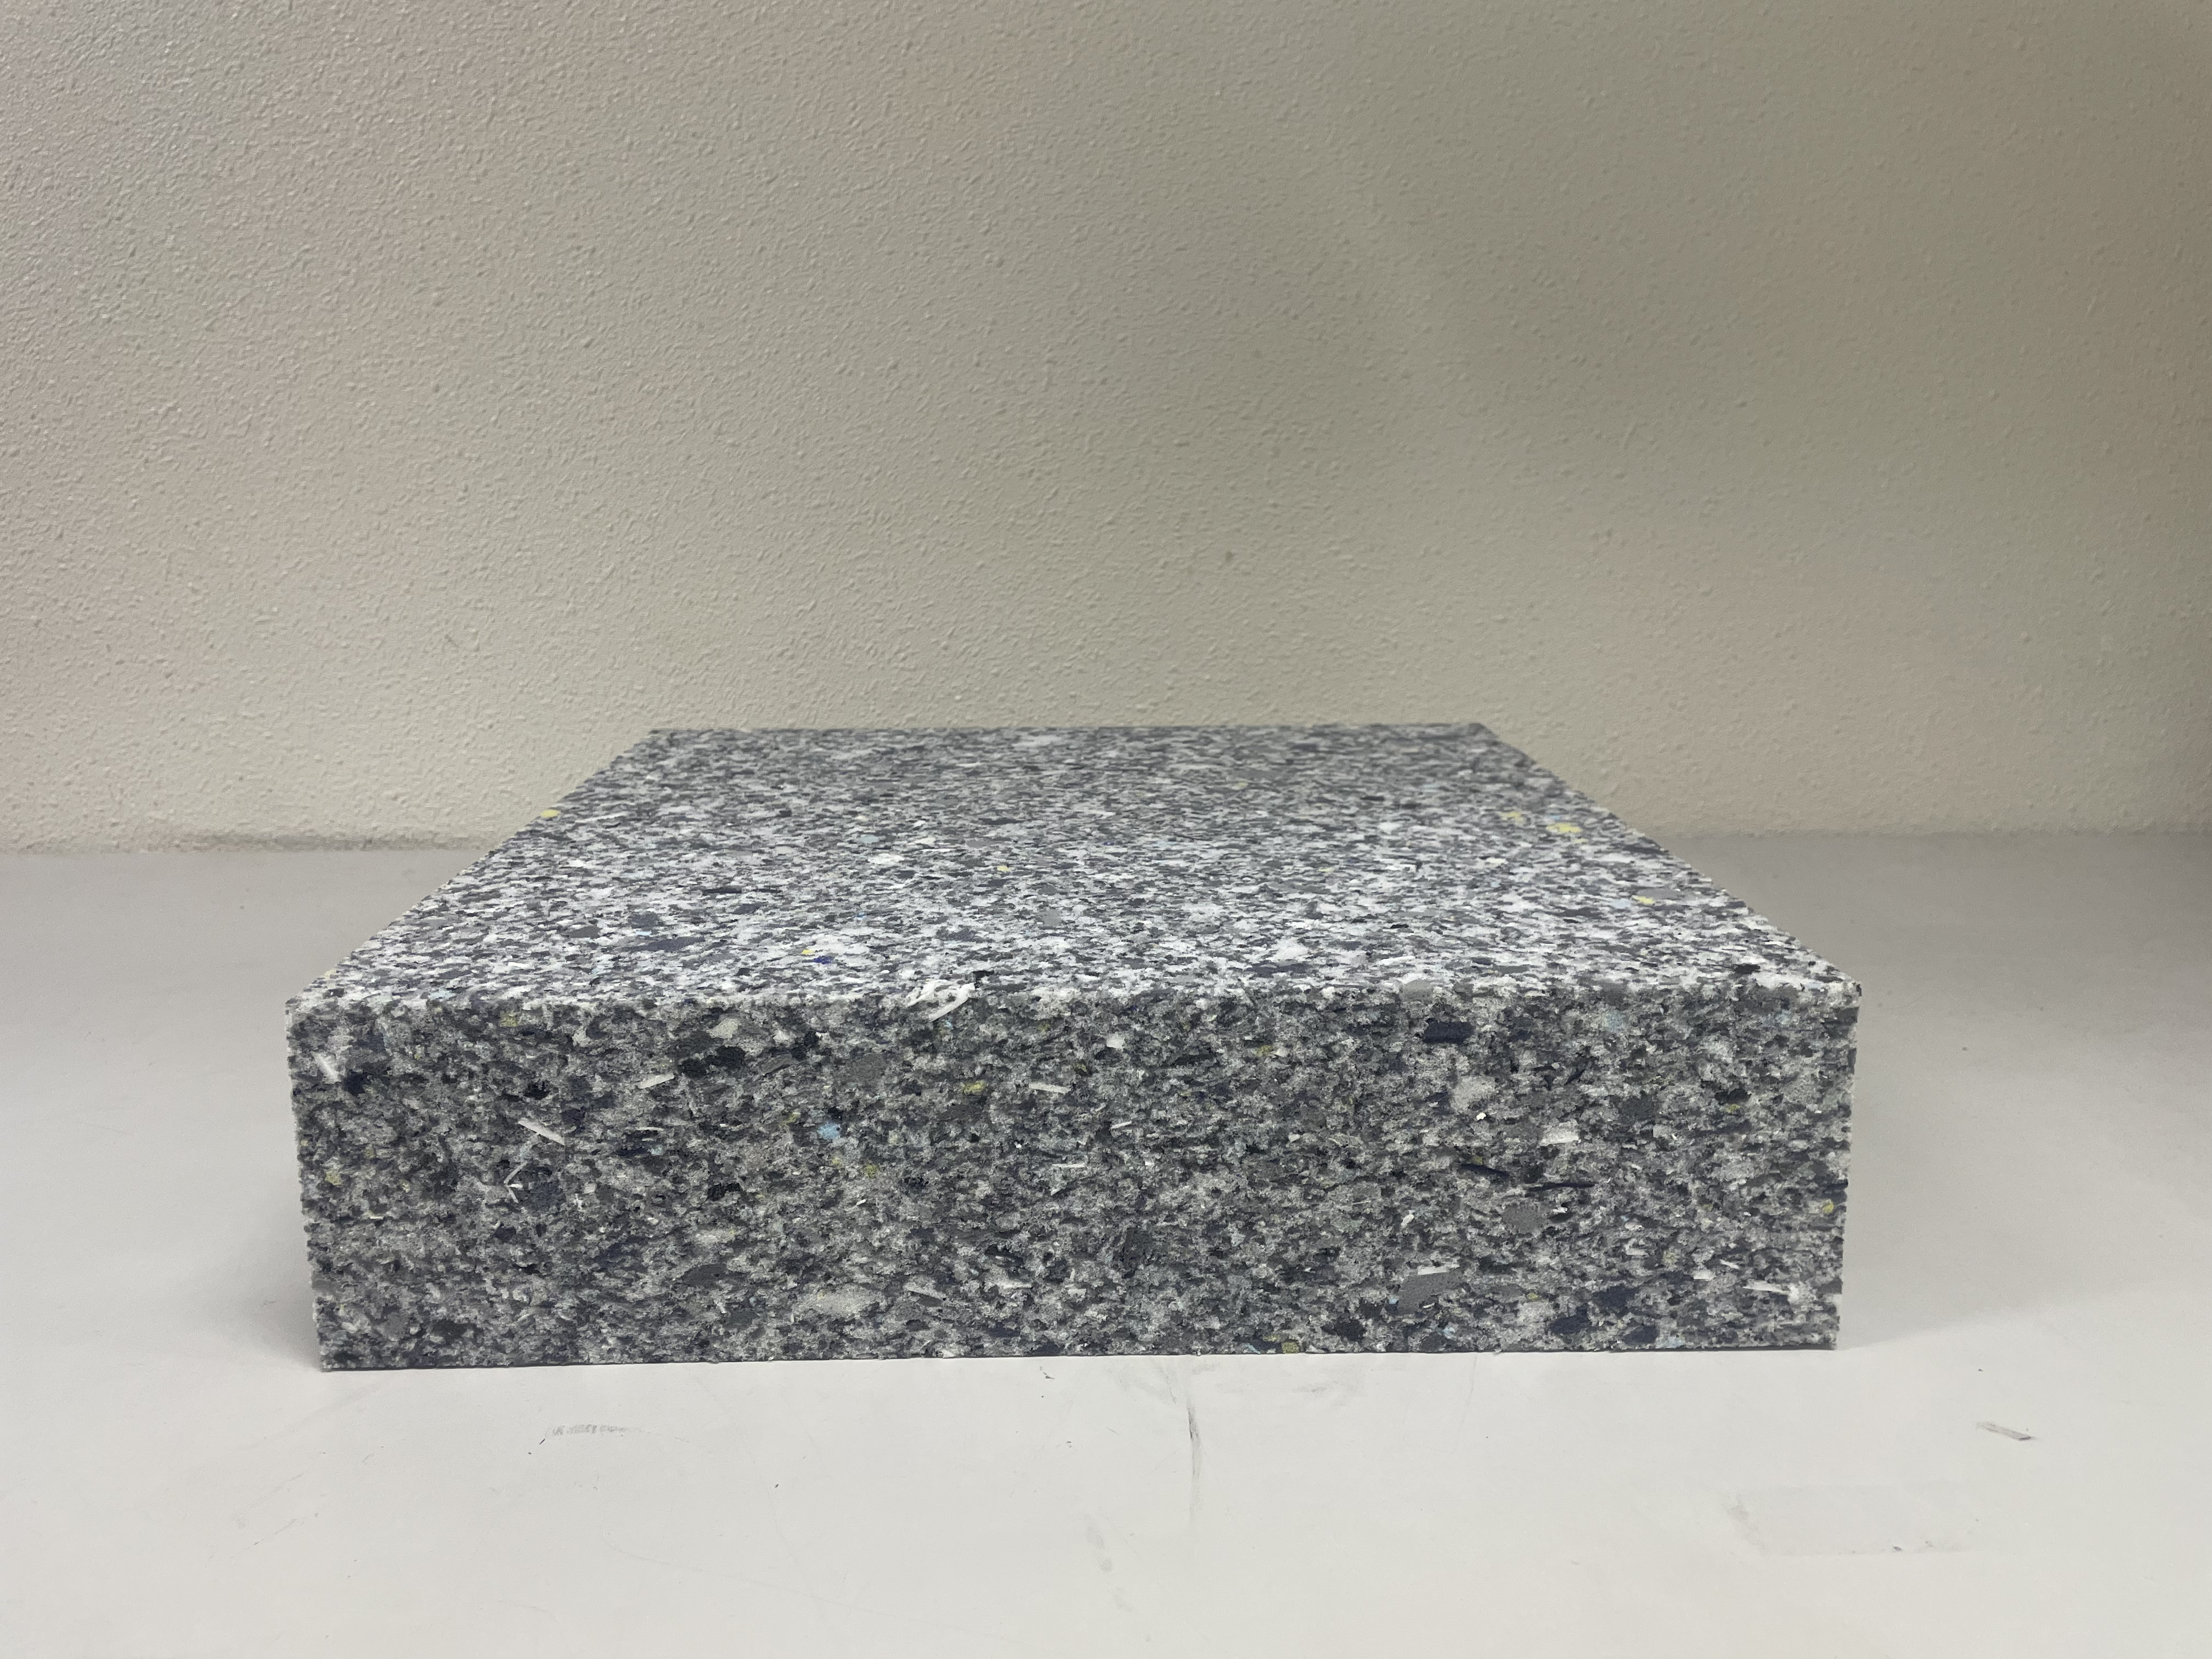
\includegraphics[width=0.5\linewidth]{images/uretan_1.png}
  \caption{高反発ウレタンの試験片}
  \label{fig:uretan_1}
\end{figure}

\begin{figure}[htbp]
  \centering
  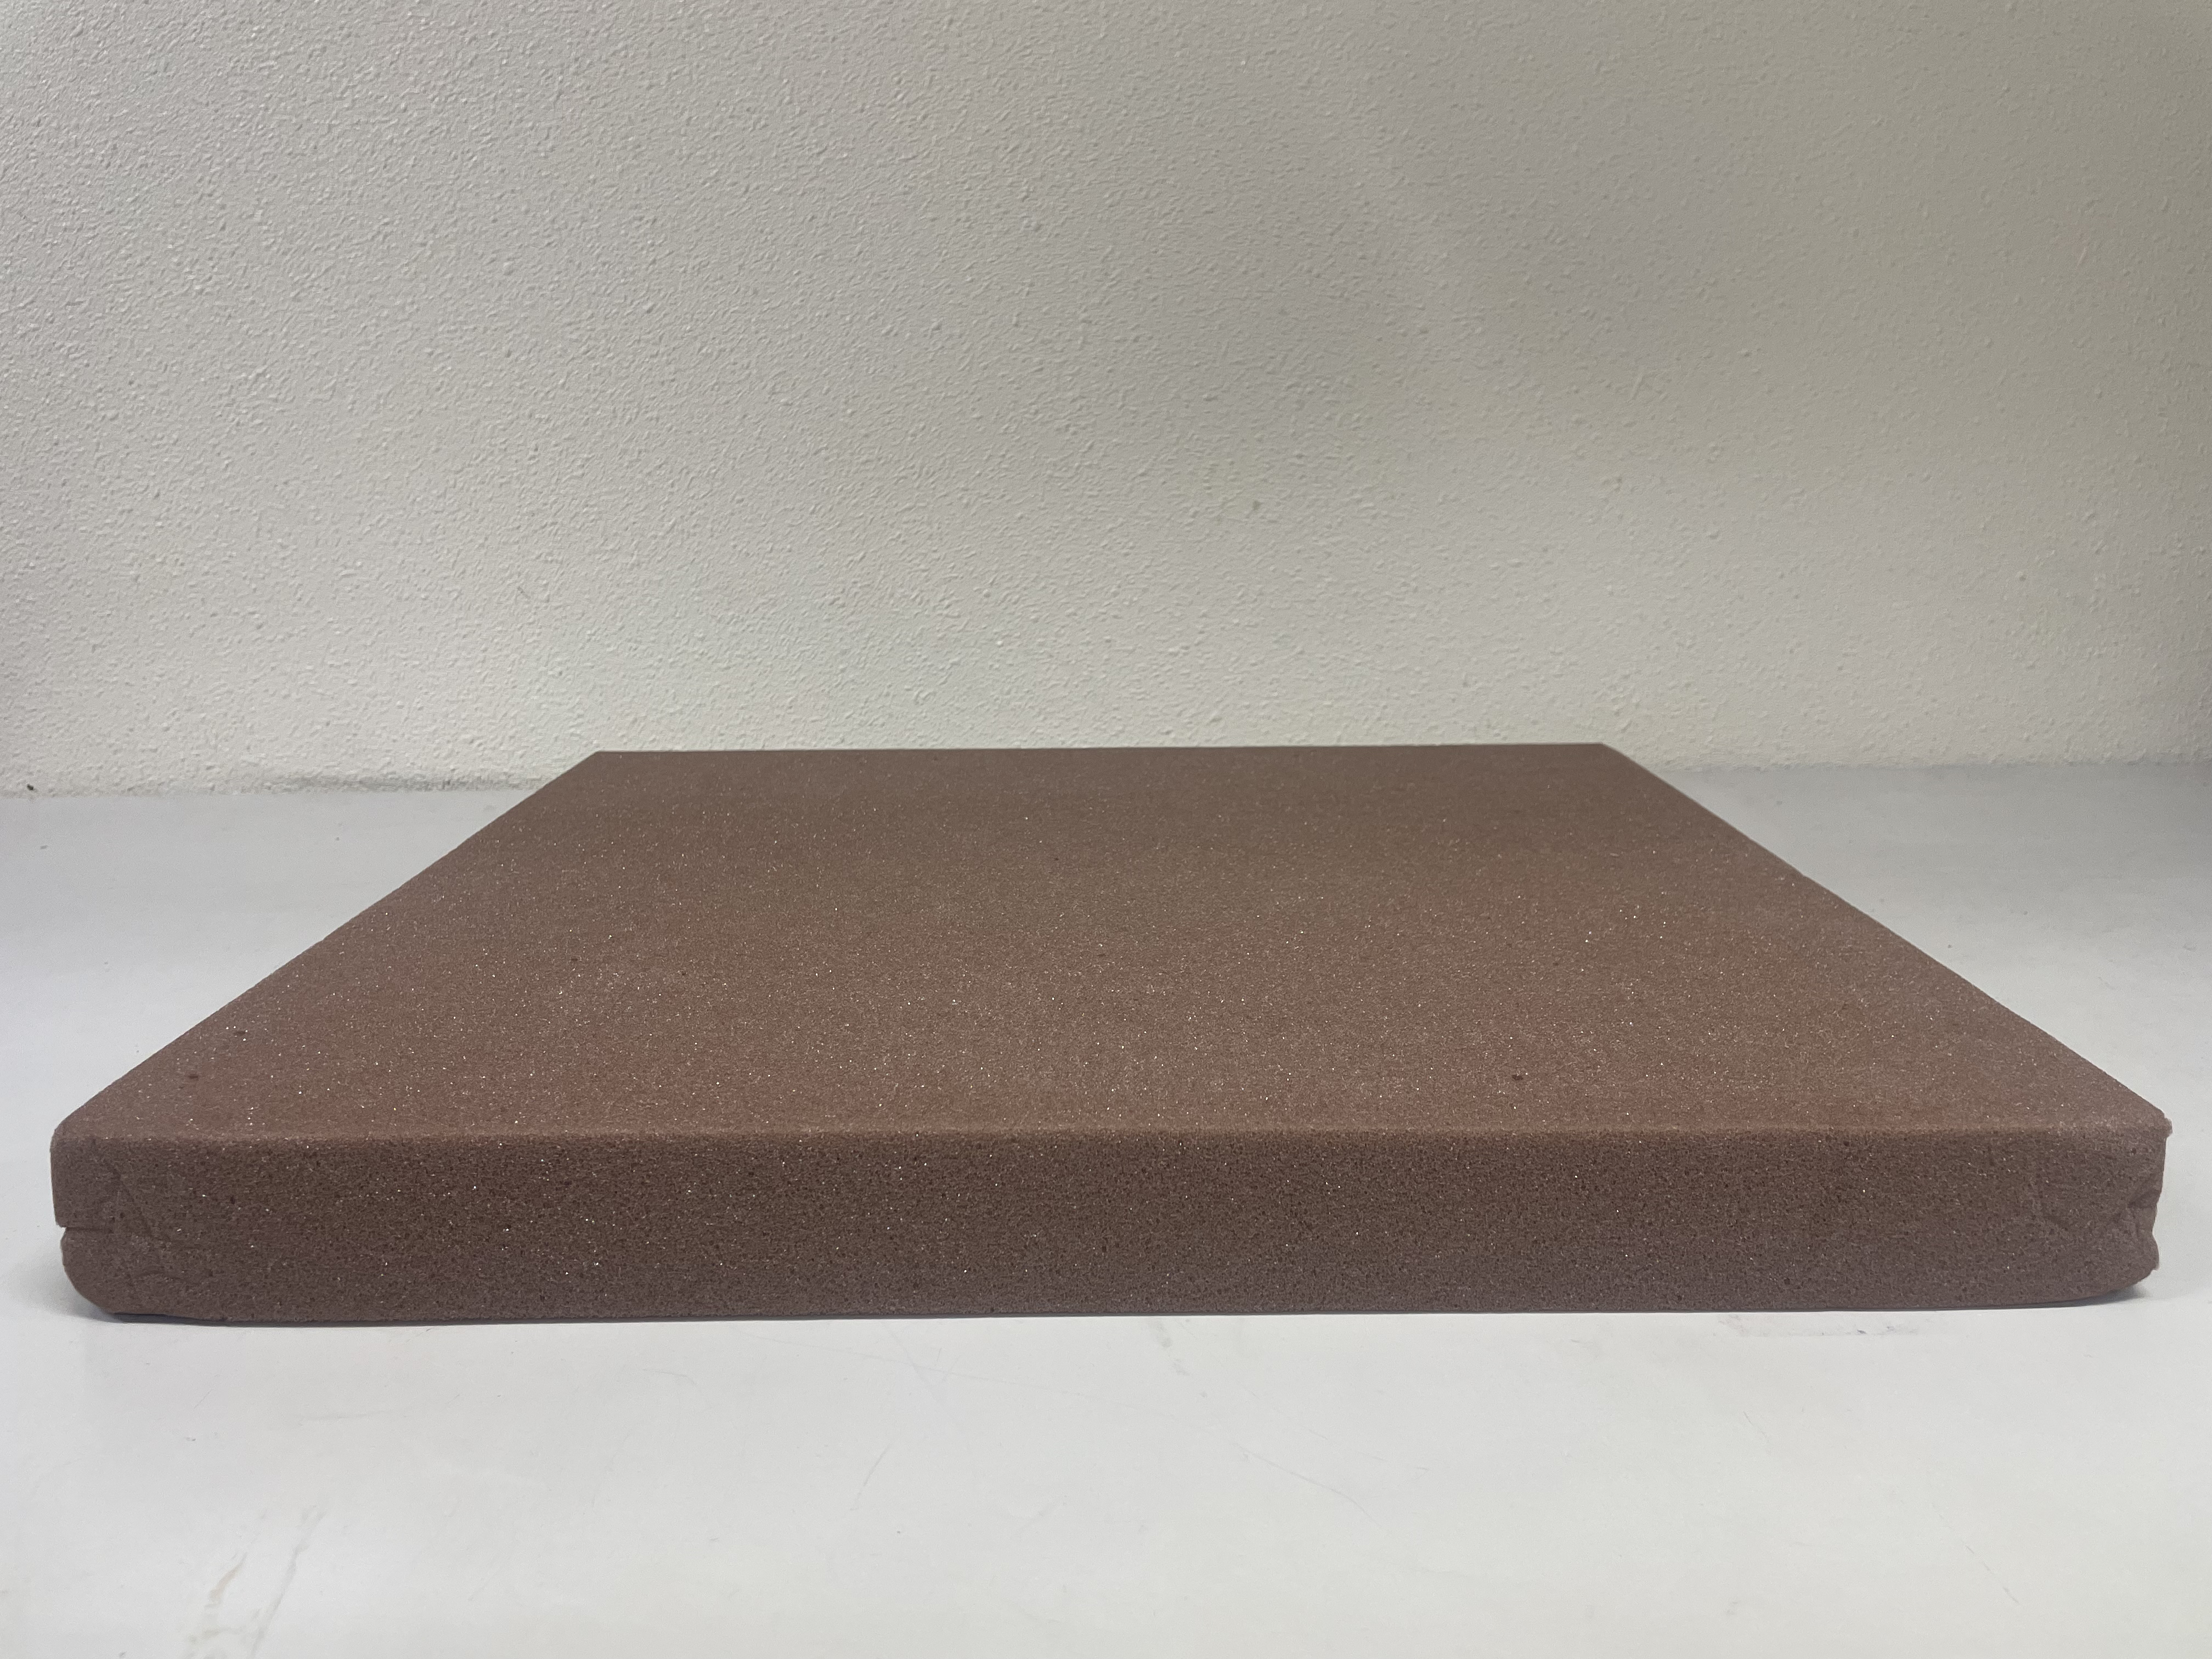
\includegraphics[width=0.5\linewidth]{images/uretan_2.png}
  \caption{低反発ウレタンの試験片}
  \label{fig:uretan_2}
\end{figure}

\begin{figure}[htbp]
  \centering
  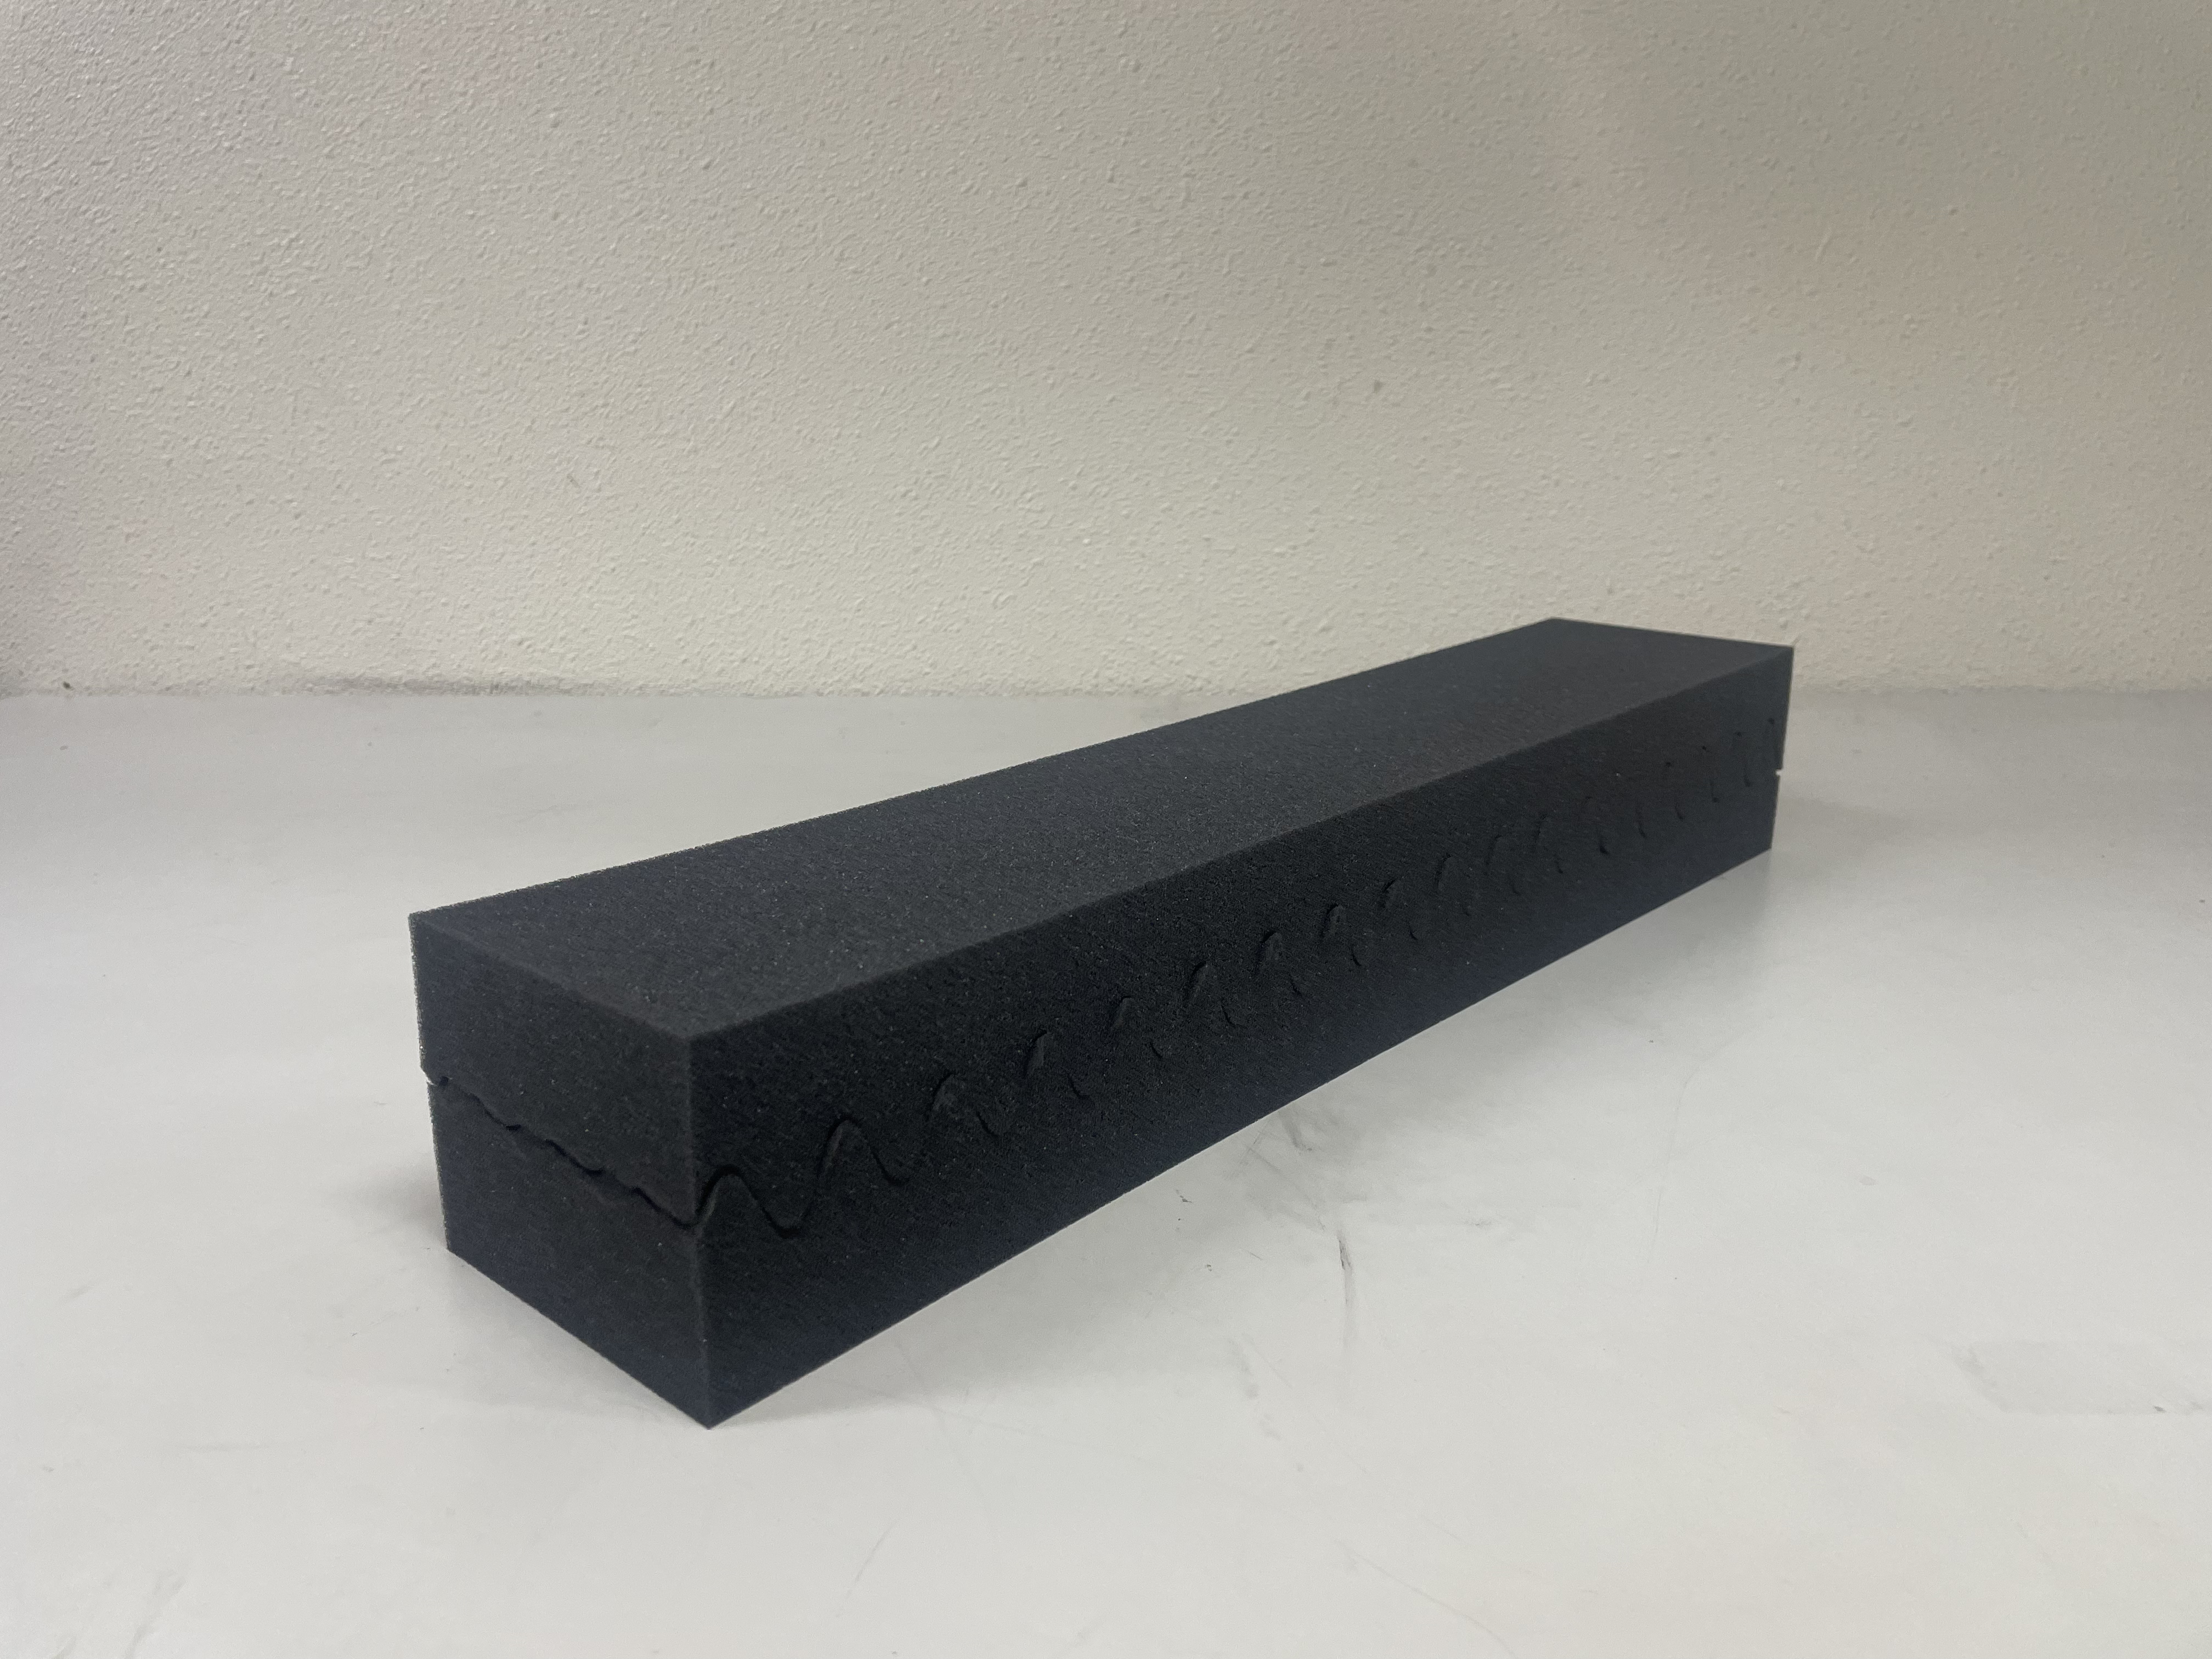
\includegraphics[width=0.5\linewidth]{images/sponzi.png}
  \caption{緩衝材スポンジ材料の試験片}
  \label{fig:sponzi}
\end{figure}